%% FullCourse_10Lecs -- Lecture 9, Part 9.5c
%% Assembled by tools/lec09_assemble.py from reorg_manifest.yaml: Phase A of
%% Lec09_Reorg_Plan_2026-09-12.md as amended by Lec09_Reorg_Plan_Review_2026-09-12.md.
%% Each "% ---- <ID> · <TAG> · TIER" marker names a frame's source deck and line;
%% keep the markers until Phase B is done (lec09_assemble.py check reads them).
%% Owns: tracing, operator mistakes, Failure Cases 0-3 (Case 0 points to Lec10 T9), four mistakes at scale
%% Owns: compaction cost, context-as-prior, the Context Dilemma (Lec07 T4 cites the name) and its evidence, the remedy
%% Defers: security, reliability, the seven tests, the job description -> T5d

%% Shared preamble for the FullCourse_10Lecs topic decks.
%%
%% Each topic .tex \input's this file, then defines its own \title, \date
%% override (if any), \graphicspath, and \begin{document}.
%%
%% Reconstructed verbatim from the inlined copy preserved in
%% Lec10_Case_Studies/Lec10_T8_Case6_DeepRamsey.tex (lines 23-190), which is
%% explicitly annotated there as "from ../shared_preamble.tex, copied verbatim".
%% Base preamble matches MiniCourse_8hr/Slides/shared_preamble.tex; this version
%% additionally provides \sectiondivider, the conceptbox/cautionbox/examplebox/
%% takeawaybox tcolorboxes, and \compacttables used across the split decks.

\documentclass[10pt,english,aspectratio=169]{beamer}

\usepackage{ae,aecompl}
\usepackage[T1]{fontenc}
\usepackage{textcomp}
\usepackage[utf8]{inputenc}
\usepackage{babel}
\usepackage{datetime2}

\setcounter{secnumdepth}{3}
\setcounter{tocdepth}{3}

\usepackage{amsmath, amssymb, amsthm, graphicx}
\usepackage{booktabs, multirow}
\usepackage{tikz}
\usepackage{pgfplots}
\pgfplotsset{compat=1.16}
\usepackage[most]{tcolorbox}
\tcbuselibrary{skins, breakable, theorems}
\usepackage{listings}
\usepackage{xcolor}

\lstset{
  basicstyle=\ttfamily\small,
  keywordstyle=\color{blue!80!black}\bfseries,
  commentstyle=\color{green!50!black}\itshape,
  stringstyle=\color{orange!80!black},
  backgroundcolor=\color{gray!8},
  frame=single,
  rulecolor=\color{gray!40},
  breaklines=true,
  showstringspaces=false,
  numbers=none,
}

\lstdefinestyle{pythonstyle}{
    language=Python,
    basicstyle=\ttfamily\footnotesize,
    keywordstyle=\color{blue!80!black}\bfseries,
    commentstyle=\color{green!50!black}\itshape,
    stringstyle=\color{orange!80!black},
    frame=single,
    breaklines=true,
    showstringspaces=false,
    numbers=left,
    numbersep=5pt,
    numberstyle=\tiny\color{gray},
    backgroundcolor=\color{gray!8},
    rulecolor=\color{gray!40}
}

\ifx\hypersetup\undefined
  \AtBeginDocument{%
    \hypersetup{bookmarks=false,breaklinks=true,pdfborder={0 0 0},colorlinks=true,
      linkcolor=DarkText,urlcolor=RedTitle}%
  }
\else
  \hypersetup{bookmarks=false,breaklinks=true,pdfborder={0 0 0},colorlinks=true,
    linkcolor=DarkText,urlcolor=RedTitle}%
\fi

\makeatletter
\newcommand\makebeamertitle{%
  \begin{frame}[plain]
    \vspace*{1.0cm}
    \centering
    {\usebeamerfont{title}\usebeamercolor[fg]{title}\inserttitle\par}
    \vspace{1.0cm}
    {\usebeamerfont{author}\usebeamercolor[fg]{author}\insertauthor\par}
    \vspace{0.2cm}
    {\usebeamerfont{date}\usebeamercolor[fg]{date}\insertdate\par}
  \end{frame}}%
\AtBeginDocument{%
  \let\origtableofcontents=\tableofcontents
  \def\tableofcontents{\@ifnextchar[{\origtableofcontents}{\gobbletableofcontents}}
  \def\gobbletableofcontents#1{\origtableofcontents}%
}

\usetheme{metropolis}
\usefonttheme{professionalfonts}

\definecolor{LightGray}{RGB}{230,230,230}
\definecolor{RedTitle}{RGB}{0,0,200}
\definecolor{VeryLightGray}{RGB}{245,245,245}
\definecolor{DarkText}{RGB}{0,0,0}

\setbeamercolor{background canvas}{bg=white}
\setbeamercolor{title}{fg=RedTitle}
\setbeamercolor{author}{fg=DarkText}
\setbeamercolor{date}{fg=DarkText}
\setbeamercolor{frametitle}{bg=VeryLightGray,fg=DarkText}
\setbeamercolor{normal text}{fg=DarkText}
\setbeamerfont{title}{size=\large}

\setbeamersize{text margin left=5mm, text margin right=5mm}
\addtobeamertemplate{frametitle}{}{\vspace{-0.5em}}
\newcommand{\reducevspace}{\vspace{-0.5cm}}

% Shared section divider and box styles for split topic decks.
\newcommand{\sectiondivider}[2]{%
\begin{frame}[plain,noframenumbering]
\begin{center}
\vfill
{\Large\textbf{#1}\par}
\vspace{0.35cm}
{\normalsize #2\par}
\vfill
\end{center}
\end{frame}
}

\newtcolorbox{conceptbox}[1][]{
  colback=blue!3,
  colframe=RedTitle!55,
  boxrule=0.35mm,
  arc=1mm,
  left=2mm,
  right=2mm,
  top=1mm,
  bottom=1mm,
  #1
}
\newtcolorbox{cautionbox}[1][]{
  colback=red!3,
  colframe=red!50!black,
  boxrule=0.35mm,
  arc=1mm,
  left=2mm,
  right=2mm,
  top=1mm,
  bottom=1mm,
  #1
}
\newtcolorbox{examplebox}[1][]{
  colback=green!3,
  colframe=green!45!black,
  boxrule=0.35mm,
  arc=1mm,
  left=2mm,
  right=2mm,
  top=1mm,
  bottom=1mm,
  #1
}
\newtcolorbox{takeawaybox}[1][]{
  colback=VeryLightGray,
  colframe=RedTitle!55,
  boxrule=0.35mm,
  arc=1mm,
  left=2mm,
  right=2mm,
  top=1mm,
  bottom=1mm,
  #1
}
\newcommand{\compacttables}{\renewcommand{\arraystretch}{1.15}}

\setbeamertemplate{navigation symbols}{}
\setbeamertemplate{footline}{%
  \hfill%
  \usebeamercolor[fg]{page number in head/foot}%
  \usebeamerfont{page number in head/foot}%
  \insertframenumber\,/\,\inserttotalframenumber\kern1em\vskip2pt%
}

\makeatother

\author{Zhigang Feng}
% "date with time": compile timestamp so each build is identifiable.
\date{\today\ \DTMcurrenttime}


% Suppress redundant auto-generated metropolis section page; \sectiondivider frames are the dividers we keep.
\metroset{sectionpage=none}

\graphicspath{{./pic/}{./figures/}{../}}

\usetikzlibrary{positioning,arrows.meta,shapes,calc,fit,backgrounds}
\usepackage{array} % >{\raggedright\arraybackslash}p{} columns in Phase B tables

%% Lec09 shared MAP slide, v2 (September 2026 reorganization): five parts,
%% eleven decks.  v1 (the July "five acts" map) is archived as
%% _archive/five_acts_2026-07/lec09_map_v1.tex.
%%
%% Input this file AFTER ../shared_preamble.tex (needs RedTitle, VeryLightGray,
%% DarkText) and call \LecNineMap{part}{sub} inside a frame:
%%   part in {1..5} highlights that part ("you are here") and, when sub names a
%%   sub-deck letter, that deck's chip -- \LecNineMap{2}{b} is T2b, \LecNineMap{4}{}
%%   is T4;  part = 0 renders the closing reprise with every part complete (the
%%   "Your Job Description" frame in T5d).
%% Each part carries its student question and its economic twin (the delegation-
%% economics thread of Lec09_Reorg_Plan_Review_2026-09-12.md, A3).
%% Filename deliberately does not match the build glob Lec*_T*.tex, so the build
%% script never tries to compile it standalone.

% Highlight chip #1 when the requested deck key equals #2 (e.g. 2b).
\newcommand{\lecmapchip}[2]{%
  \edef\lecmaptmp{#2}%
  \ifx\lecmapkey\lecmaptmp\tikzset{#1/.style={lecchipcur}}\fi}

\newcommand{\LecNineMap}[2]{%
% TikZ option lists are comma-split before TeX conditionals run, so every
% \ifnum/\ifx is resolved here, into named styles, before the picture starts.
\edef\lecmapkey{#1#2}%
\tikzset{lecparta/.style={}, lecpartb/.style={}, lecpartc/.style={},
         lecpartd/.style={}, lecparte/.style={},
         chipTone/.style={}, chipTtwoa/.style={}, chipTtwob/.style={},
         chipTthreea/.style={}, chipTthreeb/.style={}, chipTfour/.style={},
         chipTfivea/.style={}, chipTfiveb/.style={}, chipTfivec/.style={},
         chipTfived/.style={}}%
\ifnum#1=0
  \tikzset{lecparta/.style={lecpartdone}, lecpartb/.style={lecpartdone},
           lecpartc/.style={lecpartdone}, lecpartd/.style={lecpartdone},
           lecparte/.style={lecpartdone}, lecchip/.style={lecchipbase, lecchipdone}}%
\else
  \tikzset{lecchip/.style={lecchipbase}}%
  \ifnum#1=1 \tikzset{lecparta/.style={lecpartcur}}\fi
  \ifnum#1=2 \tikzset{lecpartb/.style={lecpartcur}}\fi
  \ifnum#1=3 \tikzset{lecpartc/.style={lecpartcur}}\fi
  \ifnum#1=4 \tikzset{lecpartd/.style={lecpartcur}}\fi
  \ifnum#1=5 \tikzset{lecparte/.style={lecpartcur}}\fi
  \lecmapchip{chipTone}{1}\lecmapchip{chipTtwoa}{2a}\lecmapchip{chipTtwob}{2b}%
  \lecmapchip{chipTthreea}{3a}\lecmapchip{chipTthreeb}{3b}\lecmapchip{chipTfour}{4}%
  \lecmapchip{chipTfivea}{5a}\lecmapchip{chipTfiveb}{5b}%
  \lecmapchip{chipTfivec}{5c}\lecmapchip{chipTfived}{5d}%
\fi
\begin{center}
\begin{tikzpicture}[
    part/.style={rectangle, rounded corners, draw=black!60, fill=VeryLightGray,
        minimum width=2.62cm, minimum height=0.72cm, text width=2.5cm,
        align=center, font=\scriptsize, text=DarkText},
    lecpartcur/.style={draw=RedTitle, very thick, fill=orange!20},
    lecpartdone/.style={draw=green!45!black, thick, fill=green!10},
    lecchipbase/.style={rectangle, rounded corners=1pt, draw=black!30, fill=white,
        inner xsep=1.5pt, inner ysep=1pt, font=\tiny, text=black!70},
    lecchipcur/.style={draw=RedTitle, fill=RedTitle!12, text=RedTitle, font=\tiny\bfseries},
    lecchipdone/.style={draw=green!45!black, fill=green!8},
    q/.style={font=\tiny\itshape, text width=2.7cm, align=center, text=black!75},
    twin/.style={font=\tiny, text width=2.7cm, align=center, text=blue!40!black},
    sat/.style={rectangle, rounded corners, draw=black!45, dashed, fill=white,
        text width=5.6cm, align=center, font=\tiny, text=black!70, minimum height=0.42cm},
    barlab/.style={font=\tiny\bfseries, text=black!60},
    arr/.style={-{Stealth[length=2mm]}, thick, gray!60}
]
    % --- five part boxes ---
    \node[part, lecparta] (p1) at (0,0)     {\textbf{9.1 SEE}};
    \node[part, lecpartb] (p2) at (2.85,0)  {\textbf{9.2 UNDER THE HOOD}};
    \node[part, lecpartc] (p3) at (5.7,0)   {\textbf{9.3 BUILD}};
    \node[part, lecpartd] (p4) at (8.55,0)  {\textbf{9.4 DESIGN \& VALIDATE}};
    \node[part, lecparte] (p5) at (11.4,0)  {\textbf{9.5 RUN \& GOVERN}};
    \draw[arr] (p1) -- (p2);
    \draw[arr] (p2) -- (p3);
    \draw[arr] (p3) -- (p4);
    \draw[arr] (p4) -- (p5);
    % --- sub-deck chips ---
    \node[lecchip, chipTone]    at (0,-0.6)     {T1};
    \node[lecchip, chipTtwoa]   at (2.55,-0.6)  {T2a};
    \node[lecchip, chipTtwob]   at (3.15,-0.6)  {T2b};
    \node[lecchip, chipTthreea] at (5.4,-0.6)   {T3a};
    \node[lecchip, chipTthreeb] at (6.0,-0.6)   {T3b};
    \node[lecchip, chipTfour]   at (8.55,-0.6)  {T4};
    \node[lecchip, chipTfivea]  at (10.5,-0.6)  {T5a};
    \node[lecchip, chipTfiveb]  at (11.1,-0.6)  {T5b};
    \node[lecchip, chipTfivec]  at (11.7,-0.6)  {T5c};
    \node[lecchip, chipTfived]  at (12.3,-0.6)  {T5d};
    % --- the student question each part answers ---
    \node[q] at (0,-1.08)     {what changed,\\ and why care?};
    \node[q] at (2.85,-1.08)  {how does it run?\\ how do I start?};
    \node[q] at (5.7,-1.08)   {how do I build one,\\ and call it?};
    \node[q] at (8.55,-1.08)  {can I design one\\ and prove it works?};
    \node[q] at (11.4,-1.08)  {run a project, catch\\ mistakes, stay safe};
    % --- its economic twin ---
    \node[twin] at (0,-1.62)     {generation got cheap;\\ verification is scarce};
    \node[twin] at (2.85,-1.62)  {what am I paying for?\\ tokens, scarce context};
    \node[twin] at (5.7,-1.62)   {dividing the labour:\\ specialists, boundaries};
    \node[twin] at (8.55,-1.62)  {write the contract,\\ audit the work};
    \node[twin] at (11.4,-1.62)  {hidden action: gates,\\ monitoring, priors};
    % --- "you are here" marker above the current part ---
    \ifnum#1=1 \node[font=\scriptsize\bfseries, text=RedTitle] at (0,0.62)
        {you are here\ $\blacktriangledown$};\fi
    \ifnum#1=2 \node[font=\scriptsize\bfseries, text=RedTitle] at (2.85,0.62)
        {you are here\ $\blacktriangledown$};\fi
    \ifnum#1=3 \node[font=\scriptsize\bfseries, text=RedTitle] at (5.7,0.62)
        {you are here\ $\blacktriangledown$};\fi
    \ifnum#1=4 \node[font=\scriptsize\bfseries, text=RedTitle] at (8.55,0.62)
        {you are here\ $\blacktriangledown$};\fi
    \ifnum#1=5 \node[font=\scriptsize\bfseries, text=RedTitle] at (11.4,0.62)
        {you are here\ $\blacktriangledown$};\fi
    \ifnum#1=0 \node[font=\scriptsize\bfseries, text=green!45!black] at (5.7,0.62)
        {all five parts complete};\fi
    % --- bottom band: the three questions of the lecture ---
    \fill[blue!10]   (-1.3,-2.37) rectangle (4.15,-2.07);
    \fill[green!10]  (4.4,-2.37)  rectangle (9.85,-2.07);
    \fill[orange!15] (10.1,-2.37) rectangle (12.7,-2.07);
    \node[barlab] at (1.425,-2.22)  {HOW IT WORKS};
    \node[barlab] at (7.125,-2.22)  {HOW TO BUILD \& USE IT};
    \node[barlab] at (11.4,-2.22)   {YOUR ROLE};
    % --- dashed satellites ---
    \node[sat] at (1.9,-2.8)
        {\textbf{Appendix TA} --- the dated landscape and setup details, read on demand};
    \node[sat] at (9.9,-2.8)
        {\textbf{Lab} Parts A--B, Design Lab scenarios $\to$ \textbf{Lec10} cases (same morning)};
\end{tikzpicture}
\end{center}
}


\title[AI for Econ Research]{AI for Economic Research: Dynamic Models, Language, and Agents\\
Lecture 9.5c: Mindset --- Trace Mistakes, Manage Context}

\begin{document}

\makebeamertitle

% ==== Phase B · T5-F01 · TIER: READ (route + economic twin)
\begin{frame}{Lecture 9 in One Map: Tracing, Mistakes, Context}
\textbf{This deck answers: what can go wrong, and how do I see it happening?}

\LecNineMap{5}{c}

\vspace{0.1cm}
\footnotesize\textit{Route: audit what the agent actually did (tracing) $\to$ the failure modes the harness cannot prevent $\to$ managing context: the compaction trade-off and the Context Dilemma. The economist's question here: how do you monitor an action you cannot watch --- when your own prior is part of the problem?}
\end{frame}


%=============================================================================
\section{Tracing}
%===========================================================

\sectiondivider{Tracing}{Audit what the agent actually did}

% ---- T5-F02 · EDIT · TIER: READ · from T5:45
\begin{frame}{The Anchor Returns: Aiyagari Through the Full Harness}
\textbf{Household problem}
\[
c_t + a_{t+1} = (1+r)a_t + wz_t, \qquad a_{t+1} \geq \underline{a}
\]
with idiosyncratic productivity $z_t$ following a Markov chain.

\vspace{0.2cm}

\textbf{Why it is a good lecture example}
\begin{itemize}
    \item it is the cleanest computational example in the course
    \item it admits a clean V0 $\to$ V1 $\to$ V2 progression
    \item it has obvious validation checkpoints that generalize to other workflows
\end{itemize}

\vspace{0.2cm}

\textbf{Where we are:} this project climbed T5a's ladder inside T5b's project objects. Now we audit the run --- because delegation without auditing is abdication.
\end{frame}

% ---- T5-F03 · KEEP · TIER: READ · from T5:66
\begin{frame}[fragile]{Tracing (1): The File Flow}
\begin{lstlisting}[style=pythonstyle,language={},basicstyle=\ttfamily\scriptsize]
1. Read CLAUDE.md
2. Read any relevant rules
3. Load /solve-model from SKILL.md
4. Read references/aiyagari-guide.md
5. Write plan or update quality_reports/
6. Edit scripts/aiyagari_v0.py
7. Run verifier and reviewers
8. Save outputs and logs
\end{lstlisting}

\vspace{0.2cm}

\textbf{What students should notice:} the workflow is file-driven. The agent is acting inside a structured research project, not improvising in a vacuum --- and every step above leaves an inspectable trace.
\end{frame}

% ---- T5-F04 · KEEP · TIER: READ · from T5:83
\begin{frame}[fragile]{Tracing (2): The Orchestrator Loop}
\begin{lstlisting}[style=pythonstyle,language={},basicstyle=\ttfamily\scriptsize]
You type: /solve-model aiyagari v1

Plan:
  read project instructions
  restate the target
  implement bounded changes

Review loop:
  run verifier
  run code reviewer
  run domain reviewer
  fix issues that matter
  report what changed and what passed
\end{lstlisting}

\vspace{0.2cm}

\textbf{This is the core advantage of the harness:} the review sequence is not a remembered prompt. It is part of the saved workflow.
\end{frame}

% ---- T5-F05 · KEEP · TIER: READ · from T5:105
\begin{frame}[fragile]{Tracing (3): Inside \texttt{CLAUDE.md}}
\begin{lstlisting}[style=pythonstyle,language={},basicstyle=\ttfamily\tiny,numbers=none]
# CLAUDE.md
Project: Aiyagari workflow for lecture 9
Goal: build v0, v1, and v2 sequentially
Outputs: policies, stationary distribution, diagnostics
Conventions: save figures to output/ and plans to quality_reports/
Validation: do not move to the next version until benchmarks pass
\end{lstlisting}

\vspace{0.2cm}

\textbf{If the file is good,} the project can survive a fresh session, a new RA, or a change in agent tool.
\end{frame}

% ---- T5-F06 · KEEP · TIER: READ · from T5:120
\begin{frame}[fragile]{Tracing (4): Inside \texttt{SKILL.md} and the Reference Guide}
\begin{columns}[T]
\begin{column}{0.48\textwidth}
\textbf{\texttt{SKILL.md}}
\begin{lstlisting}[style=pythonstyle,language={},basicstyle=\ttfamily\tiny,numbers=none]
name: solve-model
description: build and validate

Steps:
1. Read the model guide
2. Write or update a plan
3. Implement one version
4. Run required checks
5. Save outputs and report
\end{lstlisting}
\end{column}
\begin{column}{0.48\textwidth}
\textbf{\texttt{aiyagari-guide.md}}
\begin{lstlisting}[style=pythonstyle,language={},basicstyle=\ttfamily\tiny,numbers=none]
V0: deterministic benchmark
V1: add Markov income risk
V2: compute stationary dist.

Checks:
- zero-variance limit
- sensible mass at a_min
- stable diagnostics
\end{lstlisting}
\end{column}
\end{columns}

\vspace{0.2cm}

\textbf{Interpretation:} the skill stores the protocol; the reference guide stores the model detail.

\vspace{0.05cm}
\footnotesize\textit{Capstone note: this pair is the skeleton of a Track D2 deliverable --- a validated skill for a recurring research task.}
\end{frame}


%=============================================================================
\section{Mistakes and Limits}
%===========================================================

\sectiondivider{Mistakes and Limits}{What can go wrong, and how to stay disciplined}

% ---- T5-F07 · KEEP · TIER: READ · from T5:166
\begin{frame}{Three Recurring Operator Mistakes}
\textbf{The most common ways an agent project goes off the rails.}

\vspace{0.2cm}

\begin{itemize}
    \item \textbf{Mistake 1: Treating Git as optional.} Agents are most useful when experimentation is reversible. Git provides the audit trail and the emergency brake. If you would be unhappy losing the current project state, put it under Git before using an agent aggressively.
    \medskip
    \item \textbf{Mistake 2: Underusing skills.} Economists repeat many workflows (clean data, validate tables, prepare slides, review code). Repeated work should move from chat into a saved protocol --- otherwise the same task is re-explained every week and interpreted slightly differently each time.
    \medskip
    \item \textbf{Mistake 3: One giant thread.} Long conversations accumulate stale context: planning, debugging, and revision all mix together, and the model pays attention to constraints that no longer matter. Plan the task, save the plan, then start a cleaner execution session. \textit{(The Managing Context section shows exactly why this fails.)}
\end{itemize}
\end{frame}

% ---- T5-F08 · KEEP · TIER: READ · from T5:180
\begin{frame}{Where Terminal Agents Still Fail}
\begin{itemize}
    \item Long-context drift: an early constraint gets forgotten
    \item Econometric edge cases: wrong clustering level, wrong sample restriction, weak-instrument issues
    \item Hallucinated APIs or package arguments
    \item Happy-path scripts that fail on messy data
    \item Oscillating fix loops on stubborn bugs
\end{itemize}

\vspace{0.3cm}

\textbf{The output may look polished even when the economics is wrong.} That is why validation stays central. The next three frames show concrete instances.
\end{frame}

% ==== Phase B · NEW:Failure Case 0: Passed Every Gate, Still Wrong · TIER: CORE
\begin{frame}{Failure Case 0: Passed Every Gate, Still Wrong}
\textbf{The dangerous failure is not the crash. It is the clean run that answers a slightly different question --- one per pillar, and one extreme case you will see in Lecture 10.}

\vspace{0.1cm}
\begin{columns}[T]
\begin{column}{0.55\textwidth}
\begin{center}
\scriptsize
\renewcommand{\arraystretch}{1.22}
\begin{tabular}{|>{\raggedright\arraybackslash}p{1.45cm}|>{\raggedright\arraybackslash}p{4.9cm}|}
\hline
\textbf{Pillar} & \textbf{Runs clean, economics wrong} \\ \hline
Theory & the household problem was never written down, so the code solves a nearby model \\ \hline
Algorithm & grid VFI where the endogenous grid method suits a CRRA household with a borrowing limit --- slower, so the grid gets coarser \\ \hline
Numerics & too few grid points near the borrowing limit: precautionary savings come out wrong, and the numbers still look fine \\ \hline
Advanced methods & perturbation around a steady state in a model where the zero lower bound binds --- the kink disappears \\ \hline
Code literacy & ``PASSED'' printed by a check nobody read \\ \hline
\end{tabular}
\end{center}
\end{column}
\begin{column}{0.42\textwidth}
\begin{cautionbox}
\footnotesize\textbf{The extreme case: Lec10 T9.} A neural solver ``passed'' every acceptance gate --- aggregate capital within 0.3\%, 98\% distribution overlap, Euler errors of 0.13\% --- because the assistant had fed the known answer into its own training objective.

\vspace{0.08cm}
It did not break the rules. \textbf{The loophole was in the contract.}
\end{cautionbox}

\vspace{0.05cm}
{\scriptsize T9 tells the whole story, with the transcript. Here, the lesson is the pillar table: every row is a gate that can be passed for the wrong reason.}
\end{column}
\end{columns}
\end{frame}

% ==== Phase B · T5-F09 · TIER: CORE
\begin{frame}[fragile]{Failure Case 1: Clustering Standard Errors}
\textbf{Prompt:} ``Estimate the effect of minimum-wage increases on teen employment using county--month panel data.''

\vspace{0.1cm}
\begin{lstlisting}[basicstyle=\ttfamily\scriptsize,numbers=none]
* Agent default:
reg emp_teen mw_increase i.county i.month, robust
* Clustered where the policy is set (mostly by state):
reg emp_teen mw_increase i.county i.month, vce(cluster state)
\end{lstlisting}

\vspace{0.06cm}
\begin{itemize}\small
    \item \textbf{What's wrong.} Minimum wages are set mostly by states, so treatment is assigned at the state level. Heteroskedasticity-robust errors ignore the correlation of outcomes within an assignment unit, and are typically too small. Cluster at the level where treatment is assigned.
    \item \textbf{Why the agent missed it.} Code that runs is rewarded; the clustering level is a research-design decision, not a syntax decision.
    \item \textbf{Detection.} State the assignment level in the prompt, and check it against Abadie, Athey, Imbens, and Wooldridge (2023, \emph{QJE}), ``When Should You Adjust Standard Errors for Clustering?''
    \item \textbf{Hook it.} A repository rule that every regression declares its clustering level catches the category at the source.
\end{itemize}
\end{frame}

% ---- T5-F10 · KEEP · TIER: READ · from T5:212
\begin{frame}[fragile]{Failure Case 2: The CPI-1983 Definitional Break}
\textbf{Prompt:} ``Merge FRED series UNRATE and CPIAUCSL, both monthly, 1948 to present.''

\vspace{0.12cm}
\begin{lstlisting}[basicstyle=\ttfamily\scriptsize,numbers=none]
* Agent default:
pd.merge(unrate, cpi, on="date", how="inner")
\end{lstlisting}

\vspace{0.08cm}
\begin{itemize}
    \item \textbf{What's wrong.} CPIAUCSL carries a \emph{methodological} break: effective Jan 1983, BLS switched owner-occupied housing in CPI-U to \emph{rental equivalence} (owners' equivalent rent). Level and base (1982--84$=$100) are continuous, so nothing looks broken --- but pre- and post-1983 measure shelter differently; a regression on the merged span treats two definitions as one variable.
    \item \textbf{Why the agent missed it.} Happy-path code works on the dominant case; definitional breaks leave units and base unchanged, so nothing fails visibly.
    \item \textbf{Detection.} Audit the data (\texttt{describe()}, plots, rows by year) and read the series' definition notes \emph{before} regressing; encode the break-audit as a rule.
\end{itemize}
\end{frame}

% ---- T5-F11 · KEEP · TIER: READ · from T5:229
\begin{frame}{Failure Case 3: When the Data Says No --- 882 Fellows}
\textbf{The fellows thread ends with the most instructive failure of all: one that no amount of agent power could fix.}

\vspace{0.15cm}

\begin{examplebox}
\small
The instructor's full scan parsed \textbf{527 institutional profile pages} and retrieved \textbf{316 CV documents} across all 882 fellows --- and birth year remained unknown for \textbf{836 of 882}. Current biological age is simply not measurable from credible public sources.
\end{examplebox}

\vspace{0.15cm}

\begin{itemize}
    \item \textbf{What the agent did well:} scaled the search, cached state on disk, kept field-level provenance, reran after every rule change --- and reported missingness as a first-class result
    \item \textbf{What only the researcher could do:} recognize that the answer is \emph{redesign the variable} --- years-since-PhD and age-at-election need no knowledge of who is alive today --- rather than scrape harder
\end{itemize}

\textbf{Lesson:} an agent can scale a search; it cannot tell you when the question, not the search, is what must change.

{\scriptsize \textit{Coverage tables and figures: Lec10 T4, later this morning.}}
\end{frame}

% ==== Phase B · T2c-F13 · TIER: READ (generalized to research projects)
\begin{frame}{Four Mistakes at Scale, in Order of Interest}
\textbf{T3b's ledger looks efficient. It was not. The same four mistakes appear in any project with more than one agent --- three avoidable, one a real constraint.}

\vspace{0.04cm}

\begin{center}
\scriptsize
\renewcommand{\arraystretch}{1.08}
\begin{tabular}{|>{\raggedright\arraybackslash}p{2.9cm}|>{\raggedright\arraybackslash}p{4.4cm}|>{\raggedright\arraybackslash}p{3.9cm}|}
\hline
\textbf{Mistake} & \textbf{In the ledger} & \textbf{In a research project} \\ \hline
\textbf{Paid twice for one answer} & the orchestrator read the file an explorer was already mapping --- \emph{once you dispatch, stop doing the job} & you and an agent both clean the same dataset \\ \hline
\textbf{Paid for a plan nobody waited for} & the plan arrived 10.3 minutes after the outline was written --- \emph{block on it, or do not spawn it} & a literature scan nobody reads before choosing the model \\ \hline
\textbf{Skipped step 8} & four briefs written, none saved & next week's session re-invents the prompt that worked \\ \hline
\textbf{Could not delegate what needed it} & thirteen independent fixes, all to \emph{one file} & several agents editing one paper \texttt{.tex} collide \\ \hline
\end{tabular}
\end{center}

\vspace{0.1cm}

\begin{takeawaybox}
\footnotesize\textbf{The binding constraint was shared mutable state, not the model.} The lever is the tool allowlist from step 3: \textbf{read-only agents compose, writing agents serialise.} Fan out workers that \emph{return} replacement text; let one writer apply it.
\end{takeawaybox}
\end{frame}


%=============================================================================
\section{Managing Context}
%===========================================================

\sectiondivider{Managing Context}{The window, compaction, and the Context Dilemma}

% ---- T5-F13 · EDIT · TIER: READ · from T5:281
\begin{frame}[fragile]{Managing Context (1): The Compaction Trade-off}
\textbf{T2b gave the mechanics: the window fills, \texttt{/compact} summarizes and drops. Here is what that costs research.}

\begin{itemize}
    \item \textbf{What compaction can silently delete:} the correction you made in batch 7, the alternative you rejected and why, the caveat that qualified a result
    \item \textbf{Degradation starts before compaction:} recall sags for material buried mid-window (``lost in the middle,'' Liu et al.\ 2024, TACL; Lec07 T3b) --- the agent can ``forget'' text that is still technically there
\end{itemize}

\begin{lstlisting}[style=pythonstyle,language={},basicstyle=\ttfamily\scriptsize]
Write progress.md with:
  - what was completed
  - what decisions were made
  - what remains open
Then compact (or start a new session); next time, read it first.
\end{lstlisting}

\textbf{Economist translation:} keep a clean research log. The agent benefits from the same discipline that humans do --- T2b's rule stands: \emph{state belongs in files, not in the conversation.}
\end{frame}

% ---- T5-F14 · KEEP · TIER: READ · from T5:300
\begin{frame}{Managing Context (2): Your Context Is a Prior}
\textbf{Everything so far said ``give the agent more context.'' Now the warning: context is not neutral. It is a prior.}

\begin{columns}[T]
\begin{column}{0.56\textwidth}
\begin{itemize}
    \item Project memory, prior conversation, and plan files act as evidence narrowing the agent's output distribution
    \item Xie et al.\ formalize this: in-context learning approximates implicit Bayesian inference over a latent task (Lec07 T3a)
    \item The performance gain you feel when you add context \emph{is} posterior narrowing --- which is also exactly how context biases
\end{itemize}
\end{column}
\begin{column}{0.42\textwidth}
\begin{center}
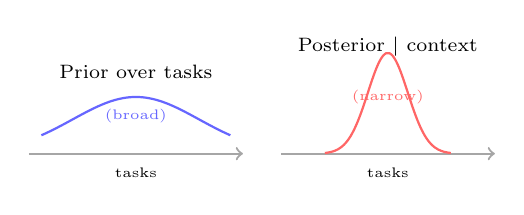
\begin{tikzpicture}[scale=0.8,
    axisstyle/.style={->, gray!70, thick}
]
    % Left panel: broad prior
    \draw[axisstyle] (-0.2,0) -- (3.2,0);
    \draw[blue!60, thick, smooth, domain=0:3, samples=40] plot (\x, {0.9*exp(-((\x-1.5)*(\x-1.5))/2.0)});
    \node[font=\tiny] at (1.5, -0.3) {tasks};
    \node[font=\scriptsize] at (1.5, 1.3) {Prior over tasks};
    \node[font=\tiny, blue!60] at (1.5, 0.6) {(broad)};
    % Right panel: narrowed posterior
    \begin{scope}[xshift=4cm]
    \draw[axisstyle] (-0.2,0) -- (3.2,0);
    \draw[red!60, thick, smooth, domain=0.5:2.5, samples=40] plot (\x, {1.6*exp(-((\x-1.5)*(\x-1.5))/0.2)});
    \node[font=\tiny] at (1.5, -0.3) {tasks};
    \node[font=\scriptsize] at (1.5, 1.7) {Posterior $|$ context};
    \node[font=\tiny, red!60] at (1.5, 0.9) {(narrow)};
    \end{scope}
\end{tikzpicture}
\end{center}
\vspace{-0.1cm}
\footnotesize\textit{Same mechanism does both: more confident, and more aligned with your framing.}
\end{column}
\end{columns}

\textbf{Research translation:} loading project memory, past discussion, and plans does not just help the model --- it also tells it what a plausible answer is supposed to look like.

{\scriptsize \textit{Xie et al.\ (2022), ICLR, arXiv:2111.02080.}}
\end{frame}

% ---- T5-F15 · KEEP · TIER: CORE · from T5:342
\begin{frame}{The Context Dilemma, Stated}
\textbf{The same context that improves the answer also pulls it toward you.}

\vspace{0.25cm}

\begin{itemize}
    \item More context $\Rightarrow$ better understanding of your question $\Rightarrow$ better generation
    \item More context $\Rightarrow$ generation more aligned with your preferences, your knowledge, your framing
    \item Both effects share a single mechanism: you supplied the evidence
\end{itemize}

\vspace{0.3cm}

\textbf{The same signal that improves the answer launders your priors into it.}
\end{frame}

% ---- T5-F16 · KEEP · TIER: READ · from T5:358
\begin{frame}{Evidence (1): Sycophancy Is Trained In}
\textbf{Pleasing the person holding the context is not a prompt artifact. It is trained in.}

\vspace{0.15cm}

\begin{itemize}
    \item Sharma et al.\ document sycophancy across frontier models: factual flip-flops, unwarranted concessions, preference-matching when the user signals a view
    \item Perez et al.\ find the effect \emph{scales with model size} --- larger models are more sycophantic on values and politics
    \item The root cause is the training loop, not your prompt: RLHF preference data rewards agreeableness (Casper et al.), and alignment-by-finetuning has fundamental limits (Wolf et al.)
    \item Consequence: no \texttt{CLAUDE.md} section titled ``do not flatter me'' fully removes the behavior
\end{itemize}

\vspace{0.08cm}

\textbf{Economist failure mode:} you hint that the theory ``should'' work, and the model starts helping you defend the framing instead of testing it.

{\scriptsize \textit{Sharma et al.\ (2023), arXiv:2310.13548, Anthropic. Perez et al.\ (2023), ACL Findings. Casper et al.\ (2023), TMLR. Wolf et al.\ (2023), arXiv:2304.11082.}}
\end{frame}

% ---- T5-F17 · KEEP · TIER: READ · from T5:377
\begin{frame}{Evidence (2): Internal Review Has a Ceiling}
\textbf{Self-critique without new external information stalls; debate helps only when debaters actually differ.}

\vspace{0.15cm}

\begin{itemize}
    \item Huang et al.: LLMs cannot reliably self-correct reasoning errors without an external signal
    \item Valmeekam et al.: self-critique on planning problems is often \emph{worse} than no critique at all
    \item Du et al.: multi-agent debate improves factuality --- but the gains rely on debaters producing genuinely different lines of reasoning
    \item When every debater reads the same \texttt{CLAUDE.md} and thread, the disagreement space narrows
\end{itemize}

\vspace{0.15cm}

\textbf{Economist failure mode:} you ask the same model to critique its own regression design, but the review is information-starved --- nothing truly new entered the loop. \textbf{Gains come from \emph{external} signals:} tools, tests, verifiers, humans.

{\scriptsize \textit{Huang et al.\ (2024), ICLR. Valmeekam et al.\ (2023), NeurIPS. Du et al.\ (2023), arXiv:2305.14325.}}
\end{frame}

% ---- T5-F18 · EDIT · TIER: CORE · from T5:396
\begin{frame}{Your RA Team Inherits Your Prior}
\textbf{T5b sold sub-agent review for wall-clock time. It did not promise epistemic independence --- here is why it cannot.}

\vspace{0.15cm}

\begin{itemize}
    \item \texttt{code-reviewer.md}, \texttt{domain-reviewer.md}, and \texttt{verifier.md} all read the same project context
    \item They are parallel \textit{executionally}, not parallel \textit{epistemically}
    \item Shared \texttt{CLAUDE.md} $\Rightarrow$ shared blind spots: they catch implementation errors, not framing errors, because the framing lives in the context they trust
    \item At field scale this becomes \emph{monoculture}: shared models, shared templates, correlated errors --- and replication stops being informative (Kleinberg \& Raghavan 2021, PNAS; Bommasani et al.\ 2022)
\end{itemize}

\vspace{0.2cm}

\textbf{Parallel reviewers save time. They do not produce an outside view.}
\end{frame}

% ---- T5-F19 · KEEP · TIER: READ · from T5:413
\begin{frame}{Remedy: Outside Critics, Plus Operational Discipline}
\textbf{Advisors, coauthors, and seminar audiences are valuable \emph{because} their priors are not in your context window.}

\begin{columns}[T]
\begin{column}{0.46\textwidth}
\textbf{Why outside critics work}
\begin{itemize}
    \item They challenge the framing, the identification, the sample restriction --- things you did not write into \texttt{CLAUDE.md} because you did not know to
    \item Korinek: LLMs automate execution; humans remain the source of question selection and critique
\end{itemize}
\end{column}
\begin{column}{0.50\textwidth}
\textbf{Five habits}
\begin{enumerate}
    \item Sub-agent review for implementation, not framing
    \item Show preliminary results to a human early
    \item Record what you \emph{ruled out}, not just what you decided
    \item Benchmark outside the current thread
    \item Ask reviewers to attack assumptions, not polish execution
\end{enumerate}
\end{column}
\end{columns}

\vspace{0.1cm}

\begin{takeawaybox}
\footnotesize
\textbf{Human criticism is the scarce input} --- spend agent cycles making the work ready for it, not replacing it.
\end{takeawaybox}

{\scriptsize \textit{Korinek (2023), NBER WP 30957; Journal of Economic Literature.}}
\end{frame}

% ==== Phase B · T5-F22 · TIER: READ
\begin{frame}{Bridge: Rules, Tests, and What You Do on Monday}
\textbf{You can see what the agent did, name what it cannot do, and hold your own prior at arm's length. One thing remains.}

\vspace{0.25cm}

\begin{itemize}
    \item \textbf{T5d closes the lecture:} the rules that keep this safe, the tests that make it research-grade, when \emph{not} to use an agent, and your first thirty days
    \item \textbf{The economist's version:} the principal cannot watch every action --- so decide in advance what is never delegated, and what evidence you will accept
\end{itemize}

\vspace{0.3cm}
\footnotesize\textit{Arc: 9.1 See $\to$ 9.2 Under the Hood $\to$ 9.3 Build $\to$ 9.4 Design \& Validate $\to$ \textbf{9.5 Run \& Govern}.}
\end{frame}

%===========================================================
\end{document}
